
\section{Karolina Surówka}
\label{seq:karsur}
I added a photo of a dog.

\begin{figure}[htbp]
    \centering
    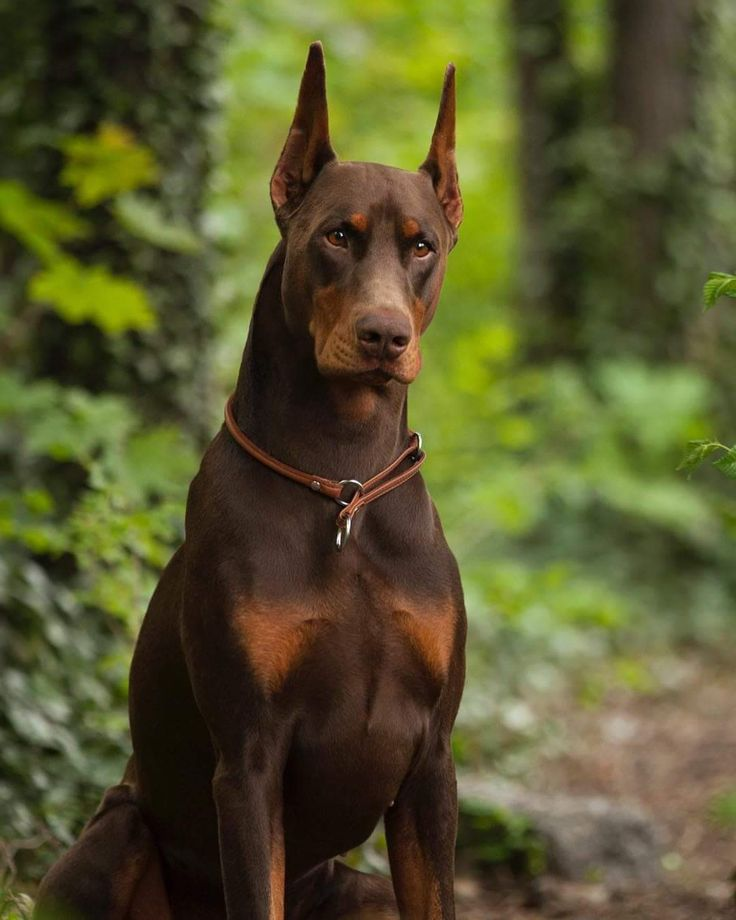
\includegraphics[width=0.4\textwidth]{Pictures/2_KSurowka.jpg}
    \caption{This is a doberman.}
 
\end{figure}

To cook chicken with rice you need:
\begin{itemize}
\renewcommand{\labelitemi}{$-$}
  \item chicken
  \item rice
  
\end{itemize}

\vspace{1.0 cm}


4 largest cities in Poland:  
\begin{enumerate}
  \item Warsaw
  \item Krakow
  \item Szczecin
  \item Lodz
\end{enumerate}


\vspace{1.0 cm}
\input{Tables/2_KSurowka_table}

\setlength{\parindent}{10ex}
 \textbf{Frederic Chopin}, the great Polish composer was born on March 1 1810 near \underline{Warsaw}.\par

\setlength{\parindent}{10ex}
 \textit{Chopin began studying music rather early. When he was only eight years old, he had already toured and had a lot of popularity in Warsaw. At this time, there were published his first works.}
 \par
\vspace{3.0 cm}







The first math equation: \(log_a b + log_a c =log_a (b*c)\).
The second one:

\begin{center}
\begin{math}
\alpha + \beta = \gamma
\end{math}
\end{center}

























